\documentclass{beamer}

\usetheme{keynote-vintage}

\usepackage{tikz}
\usetikzlibrary{shapes,arrows}

%\usepackage{fontspec}

\usepackage[utf8]{inputenc}
\usepackage[T1]{fontenc}
\usepackage{dejavu}
%\usepackage{enumitem}


\usepackage{helvet}
\renewcommand{\familydefault}{\sfdefault}

\definecolor{textcolour}{rgb}{0.37,0.34,0.27}
\definecolor{davinci}{RGB}{148,77,23}

\setbeamertemplate{background canvas}{
\includegraphics [width=\paperwidth, height=\paperheight]{pics/Vintage.png}}

\setbeamercolor{structure}{fg=textcolour}
\setbeamertemplate{items}[circle]
\setbeamerfont{structure}{family = \rmfamily}



\setbeamerfont{title}{size = \large}
\setbeamerfont{frametitle}{size = \tiny}


\usefonttheme{structuresmallcapsserif}
\usefonttheme{serif}
\setbeamercolor{normal text}{fg=textcolour}

\renewcommand{\tiny}{\fontsize{6pt}{7pt}\selectfont}
\renewcommand{\scriptsize}{\fontsize{7pt}{10pt}\selectfont}
\renewcommand{\footnotesize}{\fontsize{8pt}{10pt}\selectfont}
\renewcommand{\small}{\fontsize{10pt}{14pt}\selectfont}
\renewcommand{\normalsize}{\fontsize{10pt}{12pt}\selectfont}
\renewcommand{\large}{\fontsize{12pt}{20pt}\selectfont}
\renewcommand{\Large}{\fontsize{20pt}{33pt}\selectfont}
\renewcommand{\LARGE}{\fontsize{32pt}{43pt}\selectfont}
\renewcommand{\huge}{\fontsize{43pt}{50pt}\selectfont}
\renewcommand{\Huge}{\fontsize{76pt}{92pt}\selectfont}

\setbeamerfont{enumerate item}{size=\LARGE}
\setbeamerfont*{quote}{size=\large,shape=\itshape,series=\bfseries}
\setbeamerfont{word frame}{size=\Large, family=\rmfamily}

\newcommand{\titleframe}{
	\setbeamertemplate{background canvas}{
\includegraphics [width=\paperwidth, height=\paperheight]{pics/fond.jpg}}
	
	\begin{frame}
		\maketitle
	\end{frame}
	\setbeamertemplate{background canvas}{
\includegraphics [width=\paperwidth, height=\paperheight]{pics/Vintage.png}}
}


%%% An imageframe has one fullscreen image as background
%%% and maybe some text on top.
\newcommand{\imageframe}[2]{
%	\setbeamertemplate{background}{%
%		\parbox[c][\paperheight]{\paperwidth}{%
%			\includegraphics[width=\paperwidth,height=\paperheight]{#1}
%	}}
	\begin{frame}
		\begin{figure}[ht]
			\includegraphics[width=0.9\linewidth, height=0.8\paperheight]{pics/#1}
			\caption{\large\usebeamercolor[fg]{normal text}\centering#2}
		\end{figure}
	\end{frame}
}

%%% A wordframe has one word (or few) big and centered
\newcommand{\wordframe}[1]{
	\begin{frame}
		\bf\centering\usebeamerfont{word frame}#1
	\end{frame}
}

%%% A defnframe defines a word or phrase
\newenvironment{defnframe}[1]
{
	\begin{frame}
		\usebeamerfont{title}\usebeamercolor[fg]{box title}\Large #1: \\
		\vskip0.7cm
		\usebeamercolor[fg]{normal text}\normalsize\itshape
	}{\end{frame}}

%%% A itemframe defines a list of items
\newenvironment{itemframe}[1]
{
	\begin{frame}
		

		\usebeamerfont{title}\usebeamercolor[fg]{box title}\Large #1 \\
		\vskip0.7cm
		\usebeamercolor[fg]{normal text}\normalsize\itshape
		
	}{\end{frame}}




\def\ux{0.1\linewidth}
\def\uy{0.1\linewidth} 

\newcommand{\emptyslide}{\begin{frame}[plain]\end{frame}}

% -----------------------------------

\subject{Première Guerre Mondiale}
\title{Techniques et progrès de la médecine de guerre en 14-18}
%\subtitle{Rapport d'exposé}
\date{}
\author{\small Morine PINOT \& Christopher JACQUIOT}
\institute{Université de Caen}
\begin{document}
	\beamertemplatenavigationsymbolsempty
	%1ere de couverture
	\titleframe
	
	% introduction
	
	\section{Introduction}
	
		\begin{frame}{Introduction}
			\begin{itemize}
				\item Première guerre de cette envergure et depuis 40 ans en Europe
				\item Technologies nouvelles et non testées sur champ de bataille
				\item Médecine encore relativement peu développée en général
				\item Beaucoup de jeunes dont des médecins sont envoyés au front
				\item Beaucoup d'entre eux reviennent gravement blessés
			\end{itemize}
			
		\end{frame}
	
	% ^robematique
	
	\section{Problématique}
	
		\begin{wordframe}{De quelles façons était organisé le traitement des blessés durant la Première Guerre Mondiale?}
			
		\end{wordframe}
	
	% Sommaire
	
	\section*{Sommaire}
		
		\begin{frame}{Sommaire}
			\tableofcontents
		\end{frame}
	
	% plan detaillé
	\section{Plan détaillé}
		
		% axe 1
		
		\subsection{Les différents types de blessés}
			\begin{wordframe} {Les différents types de blessés}
			\end{wordframe}
			

		
	
			\subsubsection{Les nouvelles armes}
			
			\begin{imageframe}{I1}{De nouvelles armes}
			\end{imageframe}
			
			\subsubsection{Les nouvelles protections}
				\begin{itemframe}{De nouvelles protections}
					\begin{itemize}
						\item Masque à Gaz
						\item Casques en métal
						\item Boucliers et blindages\footnote{Dont la "pelle-bouclier" MacAdam des canadiens}
					\end{itemize}
			 	\end{itemframe}
		
		
			\subsubsection{Les nouvelles blessures et maladies}
				\begin{itemframe}{De graves blessures}
					\begin{itemize}
						\item Brûlures graves
						\item Défigurations importantes 
						\item Maladies nerveuses \& mentales (ex Obusite)
						\item Blessures chimiques
						\item Maladies due au manque d'hygiène
					\end{itemize}
				\end{itemframe}
		
		% axe 2
		
		
		\subsection{La gestion des blessés sur le front}
			\begin{wordframe} {La gestion des blessés sur le front}
			\end{wordframe}
		
			\subsubsection{Le chemin d'un blessé}
				\begin{itemframe}{Le chemin d'un blessé}
					\begin{itemize}
					\item Récupération par des brancardiers ou des camarades
					\item Redirection ou soins selon gravité des blessures au postes divisionnaires
					\item Transport par camion-ambulance sous anesthésiant vers l'HOC à 15-20km du front
					\end{itemize}
				\end{itemframe}
			
			\subsubsection{Récupération des blessés au front}
			
			\begin{frame}
				\usebeamerfont{title}\usebeamercolor[fg]{box title}\Large Les soins aux tranchées \\
				\vskip0.7cm
				\usebeamercolor[fg]{normal text}\normalsize\itshape
				\begin{columns}
					\begin{column}{0.45\linewidth}
						\begin{figure}
							\setbeamertemplate{caption}{\raggedright\insertcaption\par}								
							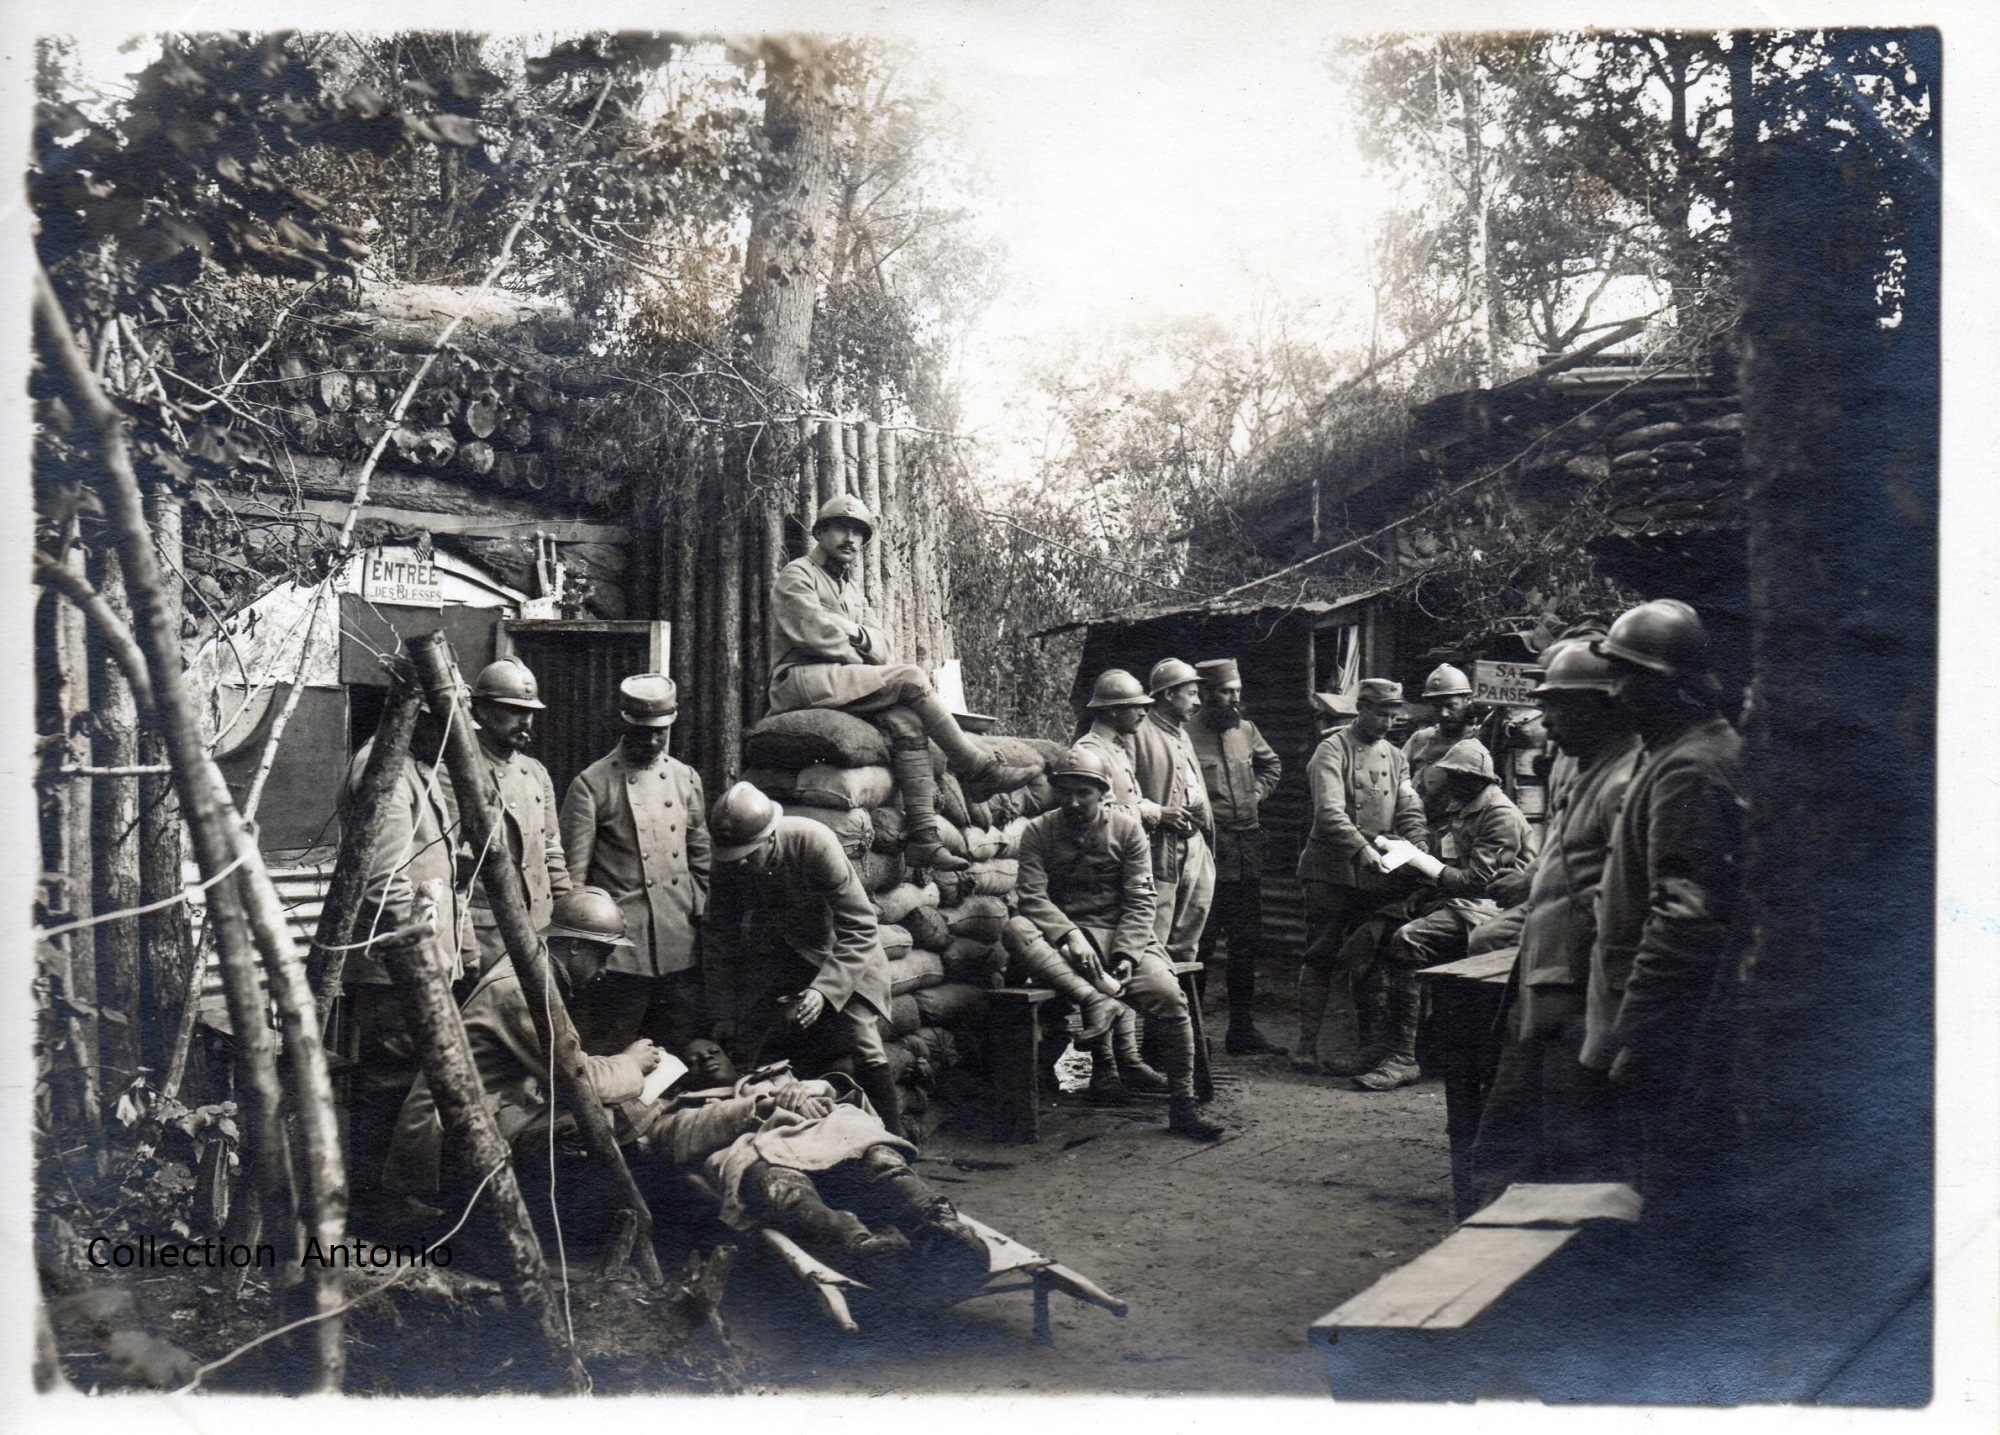
\includegraphics[width=0.8\linewidth]{pics/II2a}
							
							\caption{\tiny Poste de secours divisionnaire}
						\end{figure}
						\begin{itemize}
							\item Tri des blessés
							\item Premiers soins
						\end{itemize}
					\end{column}
					
					
					\begin{column}{0.45\linewidth}
						\begin{figure}
							\setbeamertemplate{caption}{\raggedright\insertcaption\par}								
							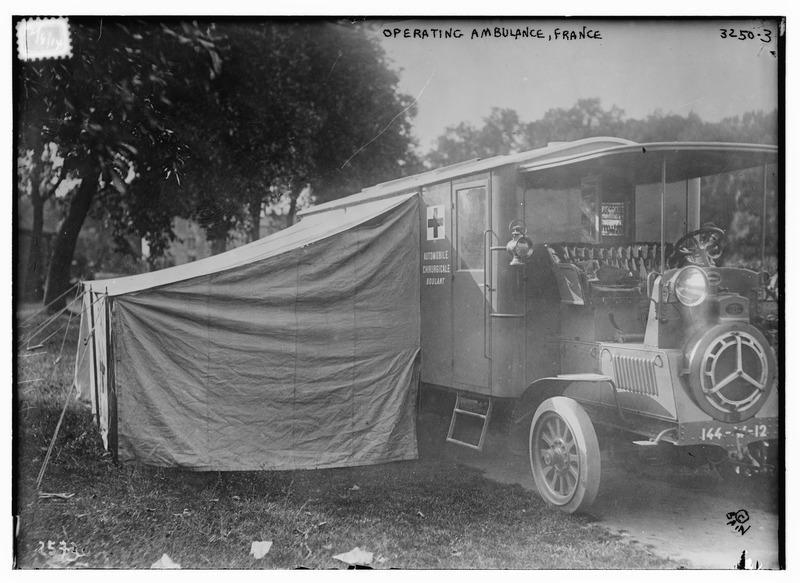
\includegraphics[width=0.8\linewidth]{pics/II2b}
							
							\caption{\tiny Ambulance chirurgicale}
						\end{figure}
						\begin{itemize}
							\item Radiologies
							\item Chirurgies basiques
						\end{itemize}
					\end{column}
				\end{columns}
					
			\end{frame}
			
			
			\subsubsection{Triage des blessés}

				\begin{frame}
					\usebeamerfont{title}\usebeamercolor[fg]{box title}\Large Triage des blessés \\
					\vskip0.7cm
					\usebeamercolor[fg]{normal text}\normalsize\itshape
					\begin{columns}
						\begin{column}{0.3\linewidth}
							\begin{figure}
								\setbeamertemplate{caption}{\raggedright\insertcaption\par}								
								
\includegraphics[width=0.8\linewidth]{pics/II3a}

								\caption{\tiny Légèrement blessé}
							\end{figure}
							\begin{itemize}
								\item Traitement minime
								\item Retourne au combat
							\end{itemize}
						\end{column}
					
						
						\begin{column}{0.3\linewidth}
							\begin{figure}
								\setbeamertemplate{caption}{\raggedright\insertcaption\par}								
								
\includegraphics[width=0.8\linewidth]{pics/II3b}
								
								\caption{\tiny Hospitalisation nécessaire}
							\end{figure}
							\begin{itemize}
								\item Premiers soins
								\item Envoyé à l'arrière
							\end{itemize}
						\end{column}
					
						
						\begin{column}{0.3\linewidth}
							\begin{figure}
								\setbeamertemplate{caption}{\raggedright\insertcaption\par}								
								
\includegraphics[width=0.8\linewidth]{pics/II3c}
								
								\caption{\tiny Blessures trop graves}
							\end{figure}
							\begin{itemize}
								\item Aucun traitement
								\item Laissé décéder
							\end{itemize}
						\end{column}
								
					\end{columns}
				\end{frame}
			
		% axe 3
		
		
		\subsection{La gestion des blessés à l'arrière}
			
			\begin{wordframe} {La gestion des blessés à l'arrière}
			\end{wordframe}
		
			\subsubsection{Logistique}
			{\begin{frame}

				\usebeamerfont{title}\usebeamercolor[fg]{box title}\Large Le trajet d'un blessé selon son état\\
				\vskip0.7cm
				\usebeamercolor[fg]{normal text}\normalsize\itshape
				\begin{columns}
				
				
					\begin{column}[t]{0.25\linewidth}
						\begin{figure}
							\setbeamertemplate{caption}{\raggedright\insertcaption\par}								
							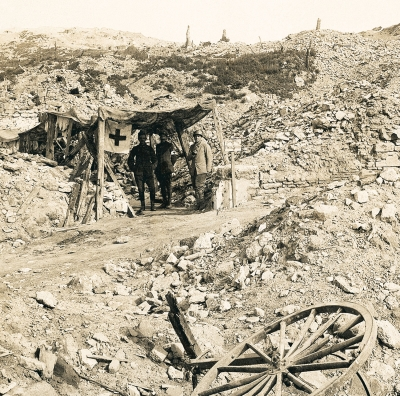
\includegraphics[width=0.8\linewidth, height=0.8\linewidth]{pics/III1b}
							
							\caption{\tiny Poste de secours}
						\end{figure}
						\begin{itemize}
							\item \tiny Départ - camion
							\item \tiny Triage des blessés et soins
						\end{itemize}
					\end{column}
				
					\begin{column}[t]{0.25\linewidth}
						\begin{figure}
							\setbeamertemplate{caption}{\raggedright\insertcaption\par}								
							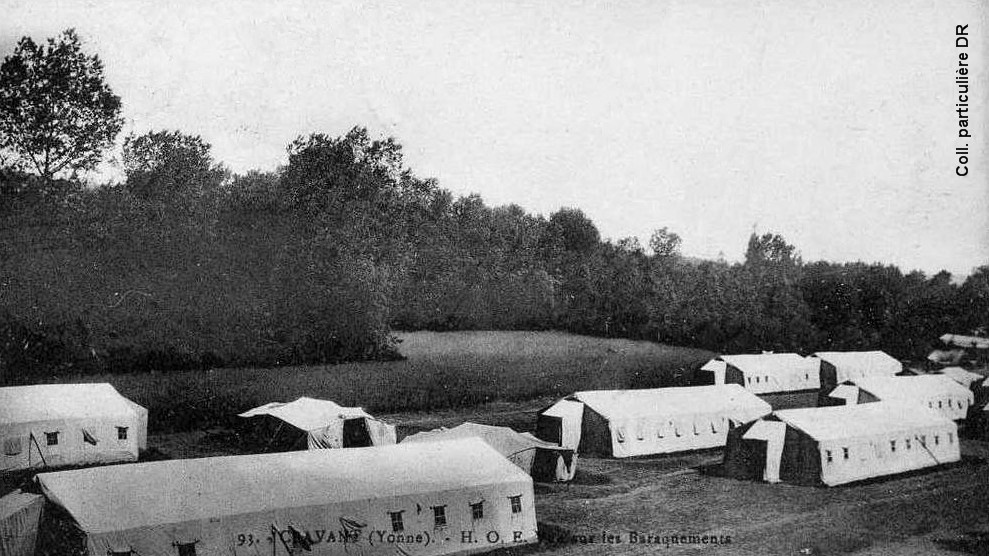
\includegraphics[width=0.8\linewidth, height=0.8\linewidth]{pics/III1c}
							
							\caption{\tiny HOE}
						\end{figure}
						\begin{itemize}
							\item \tiny Départ - train
							\item \tiny Soins des indéplaçables
						\end{itemize}
					\end{column}
				
					\begin{column}[t]{0.25\linewidth}
						\begin{figure}
							\setbeamertemplate{caption}{\raggedright\insertcaption\par}								
							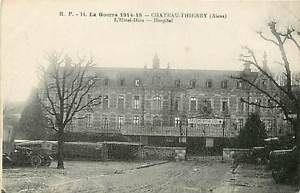
\includegraphics[width=0.8\linewidth, height=0.8\linewidth]{pics/III1d}
							
							\caption{\tiny Hôpital de campagne}
						\end{figure}
						\begin{itemize}
							\item \tiny Départ - train
							\item \tiny Soins plus avancés
						\end{itemize}
					\end{column}
				
					\begin{column}[t]{0.25\linewidth}
						\begin{figure}
							\setbeamertemplate{caption}{\raggedright\insertcaption\par}								
							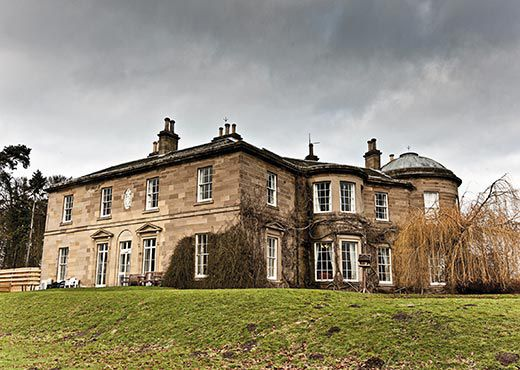
\includegraphics[width=0.8\linewidth, height=0.8\linewidth]{pics/III1e}
							
							\caption{\tiny Centre de Convalescence}
						\end{figure}
						\begin{itemize}
							\item \tiny Repos et guérison
							\item \tiny Suivi des traitements
						\end{itemize}
					\end{column}
					
				\end{columns}
			\end{frame}}
			
			
			\subsubsection{\'Evolution de l'organisation des hôpitaux}
				\begin{itemframe}{Les pratiques évoluent}
					\begin{itemize}			
						\item Apparition de nouvelles spécialisations, domaines
						\item Optimisation de l'organisation, plus de chirurgies, moins de salle, besoin de coordination
					\end{itemize}
				\end{itemframe}
				
			
			\subsubsection{Nouvelles techniques médicales}
				\begin{imageframe}{III3}{Des avancées médicales}
				\end{imageframe}
				
	% conclusion
	\section{Conclusion}
		\begin{itemframe}{Conclusion}
			De quelles façons était organisé le traitement des blessés durant la Première Guerre Mondiale?
			\begin{itemize}
				\item Gestion pragmatique des blessés dans les tranchées 
				\item Des progrès médicaux et technologiques forcés par la forte demande de soins
				\item Nouvelles spécialisations médicales dédiées à de nouveaux types de blessures
			\end{itemize}
		\end{itemframe}

\end{document}
